\chapter{Planning}
Planning combines two major areas of AI, search and logic, and representing actions and change in
logic we can cast the problem of planning as a SAT problem in the propositional case and as 
theorem planning in the case of FOL.\newline
In classical planning we will introduce a restricted language suitable for describing planning
problems and this allows to circumvent representation and computational problems by 
resorting to a restricted FOL representation.

A Planning agent has an explicit representation of the goal state, of actions and their effects,
it is able to inspect the goal and decompose it and make abstractions; it can also work freely
on the plan construction, manipulating goals and plans and some general heuristics and algorithms
for planning become possible, leveraging on this representation.

\begin{figure}
	\includegraphics[width=\textwidth]{Images/satPlan}
	\caption{Pseudocode of SatPlan approach}
	\label{img:satPlan}
\end{figure}
In figure \ref{img:satPlan} there is the pseudocode to planning as satisfiability in PROP, where
the planning problem is translated into a CNF sentence for increasing values of $t$ until a 
solution is found or the upper limit to the plan length is reached.\newline
Planning is the generation of a sequence of actions, a plan $p$, to reach the goal $G$, so
this amounts to proving that $\exists p G(Result(p, s_0))$.\newline
The Green planner used a theorem prover based on resolution and the task is made complex by 
different sources of non-determinism: the length of the sequence of actions is not known in 
advance, frame actions may infer many things that are irrelevant, we need to resort to ad hoc
strategies, we do not have any guarantee of the efficiency of the generated plan and 
a general theorem prover is inefficient and semi-decidable, so completeness is not guaranteed.

In classical planning we assume fully observable, deterministic, static environments with
single agents and we assume a factored representation, so a state of the world is represented
by a collection of variables.\newline
We use PDDL (Planning Domain Definition Language) is a specialized language for describing 
planning problems, in particular states, initial, goal states, applicable actions and 
transition model through action schemas.

In PDDL states are conjuctions/set of fluents, ground positive atoms, no variables and also
no function; database semantics is used, since we assume closed world assumption and unique
name assumption.\newline
Actions are defined by a set of action schemas that implicitly define the $Actions(s)$ and 
their result $Result(s, a)$ and actions are defined in a way that avoids the frame problem
since they require that we carefully specify all the charges and all the rest it assumed
to persist.

Action schemas correspond to parametric actions or operators and action are represented 
by the following two components:
\begin{description}
   \item [$PRECOND$: ] a list of preconditions to be satisfied in $s$ for the action to be 
	               applicable
		       \[ (a \in ACTIONS(s)) \iff s \models PRECOND(a) \]
   \item [$EFFECT$: ] the successor state $s'$ is obtained from $s$ as result of the action by
	      \[ RESULT(s, a) = (s - DEL(a)) \cup ADD(a) \]
\end{description}
In figure \ref{img:PDDLExample} is possible to note an example of PDDL actions.

\begin{figure}
	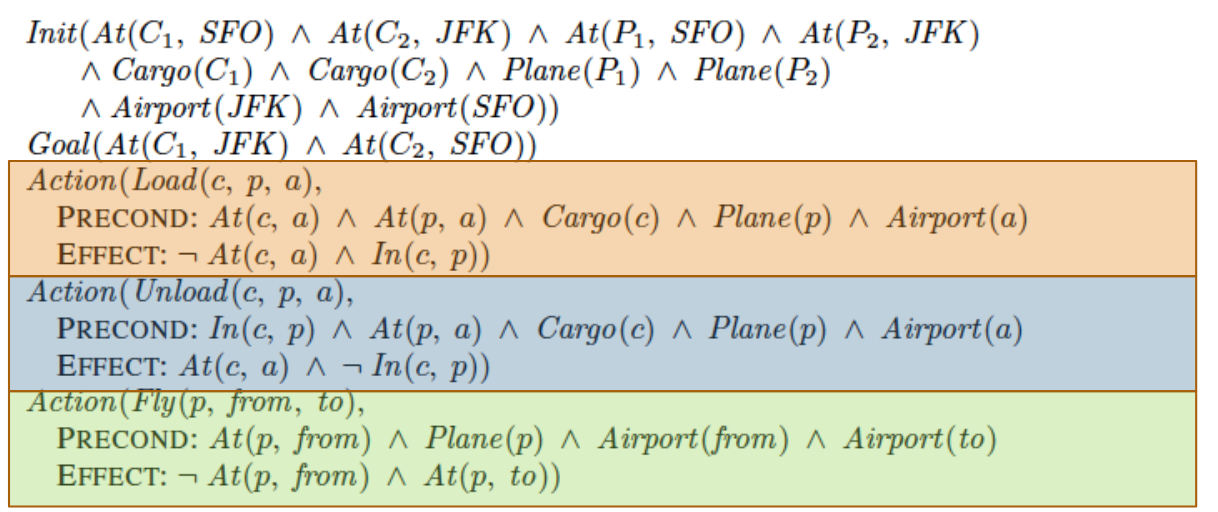
\includegraphics[width=\textwidth]{Images/PDDLEx}
	\caption{Example of PDDL actions}
	\label{img:PDDLExample}
\end{figure}
PlanSAT answer if does a plan exist, instead Bounded PlanSAT solve the problem to answer if
there is a solution of length $k$ or less.\newline
Both problems are decidable for classical planning, with PlanSAT decidable only without functions
instead Bounded PlanSAT is always decidable, also with functions.\newline
Theoretical complexity for both PlanSAT and Bounded PlanSAT is very high and if we disallow 
negative effects both problems are still NP-Hard and if we also disallow negative preconditions
PlanSAT reduces to the class P.

If we view Planning as state-space search, where nodes in the search space are states and arcs
are the actions, we have two different type of planning:
\begin{description}
    \item [Progression planning] forward search from the initial state to the goal state and it
	    is believed to be inefficient.\newline
		Prone to exploring irrelevant actions and often have large state spaces.
    \item [Regression planning ] backward search from the goal state to the initial state.
\end{description}
We start with the goal , a conjuction of literals, describing a set of worlds and the PDDL 
representation allows to regress action 
\[ g' = (g - ADD(a)) \cup Precond(a) \]
Actions that are useful to reach a goal are defined \emph{relevant} and relevant actions 
contribute to the goal but must be the last step to the solution  and given a goal $g$ containing
a literal $g_i$, an action $a$ is relevant action towards $g$ if action schema $A$ has an effect
literal $e$ such that $Unify(g_i, e) = \Theta$, $a = SUBST(\Theta, A)$ and also there is no
effect in $a$ that is the negation of a literal in $g$.\newline
One of the earlier planning system was a linear regression planner called \emph{STRIPS}.

Given the factored representation we can devise good general heuristics for planning, and 
\emph{problem relaxation} is a common technique for finding admissible heuristics, which consists
in looking at the problem with less constraints and computing the cost of the solution
in the relaxed problem.\newline
This cost can be used as an admissible heuristics for the relaxed problem and there are 
two strategies to relax the problem:
\begin{enumerate}
   \item Add more arcs to the graph, so it is easier to find a path to the goal, and 
	 \emph{Ignore preconditions heuristics} and \emph{Ignore delete list heuristics} are 
	 of this type.
   \item Group multiple nodes together, forming an abstraction of the state space 
	 (with fewer states, it is easier to search).
\end{enumerate}
The \emph{ignore preconditions} heuristic drops all preconditions from actions and every action
is applicable in any state, any single goal literal can be satisfied in one step or there 
is no solution.\newline 
The number of steps to solve a goal is approximated by the number of unsatisfied subgoals, 
but one action may achieve more than one subgoal (non admissible estimate) and one action
may undo the effect of another one (admissible).\newline
An accurate heuristics consist to remove all preconditions and all effects except those that
are literals in the goal and count the minimum number of actions required such that the 
union of those actions' effects satisfies the goal (NP-Complete but greedy approximations exist).

As an alternative we could ignore only some selected preconditions from the actions.

\emph{Ignore delete list} heuristic consist to assume that all goals and preconditions contain
only positive literals and remove the delete lists from all actions (removing all negative
literals from effects) and no action will ever undo the effect of actions, so there is a 
monotonic progress towards the goal.\newline
We use the length of the solution as admissible heuristics and is still NP-Hard to find the 
optimal solution of the relaxed problem to compute the heuristic function but this can 
be approximated in polynomial time, with hill-climbing.

In figure \ref{img:ignoreDeleteEx} is possible to see two state spaces from planning problems
with the ignore delete lists heuristic.

\begin{figure}
	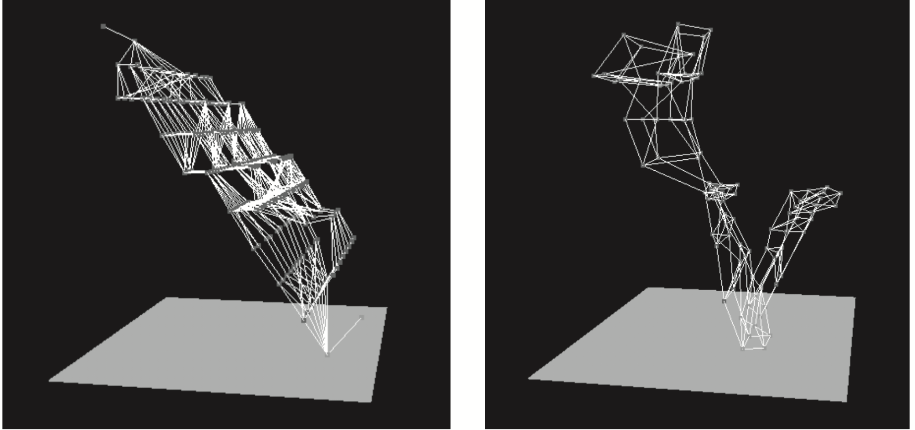
\includegraphics[width=\textwidth]{Images/ignoreDeleteEx}
	\caption{Comparison between two state space without and with ignore delete lists heuristics}
	\label{img:ignoreDeleteEx}
\end{figure}
In order to reduce the number of states, we need other forms of relaxations, so state abstractions
reduces the number of states.\newline
A state abstraction is a many-to-one mapping from states in the ground/original representation
of the problem to a more abstract representation, instead \emph{Decomposition} divide a problem
into parts, solve each part independently and then combine the subplans.\newline
The subgoals \emph{independence assumption} is that the cost of solving a conjuction of 
subgoals is approximated by the sum of the costs of solving each subgoal independently and 
this assumption can be \emph{optimistic} (admissible), when there are negative interactions,
and \emph{pessimistic} (inadmissible), when subplans contain redundant actions.\newline
Two techniques used to find useful independent sub-problems are \emph{pattern database} (
solve subproblems and memorize their cost) and \emph{hierarchical decomposition}.

A data structure commonly used in Planning is \emph{Planning Graph}, that can be used to give 
better heuristics estimates to employ in conjuction with search algorithms and it is the 
search space of an algorithm called \emph{GraphPlan}.

A search tree is exponential in size and a planning graph is a polynomial size approximation of 
the search tree and can be constructed quickly.\newline
The planning graph can't answer definitively whether $G$ is reachable from $S_0$, but it may 
discover that the goal is not reachable and can estimate how many steps it takes, in the most 
optimistic case, to reach $G$, so it can be used to derive an admissible heuristic.

Planning graphs work only for propositional planning problems, with no variables and is 
a directed graph which is built forward, organized into levels:
a level $S_0$ for the initial state, representing each fluent that holds in $S_0$, a level $A_0$ 
consisting of nodes for each ground action applicable in $S_0$ and alternating levels $S_i$
followed by $A_i$ are built until we reach a termination condition.

$S_i$ contains all the literals that could hold at time $i$ (even contrary literals $P$ and 
$\not P$) and $A_i$ contains all the actions that could have their preconditions satisfied 
at time $i$.

Mutual exclusion links (mutex) connect incompatible pairs of literals and actions:
\begin{enumerate}
	\item Mutex between literals mean that two literals cannot appear in the same belief state.
	\item Mutex between actions mean that two actions cannot occur at the same time.
\end{enumerate}
In figure \ref{img:examplePlanning} is possible to note an example of planning graph.

\begin{figure}
	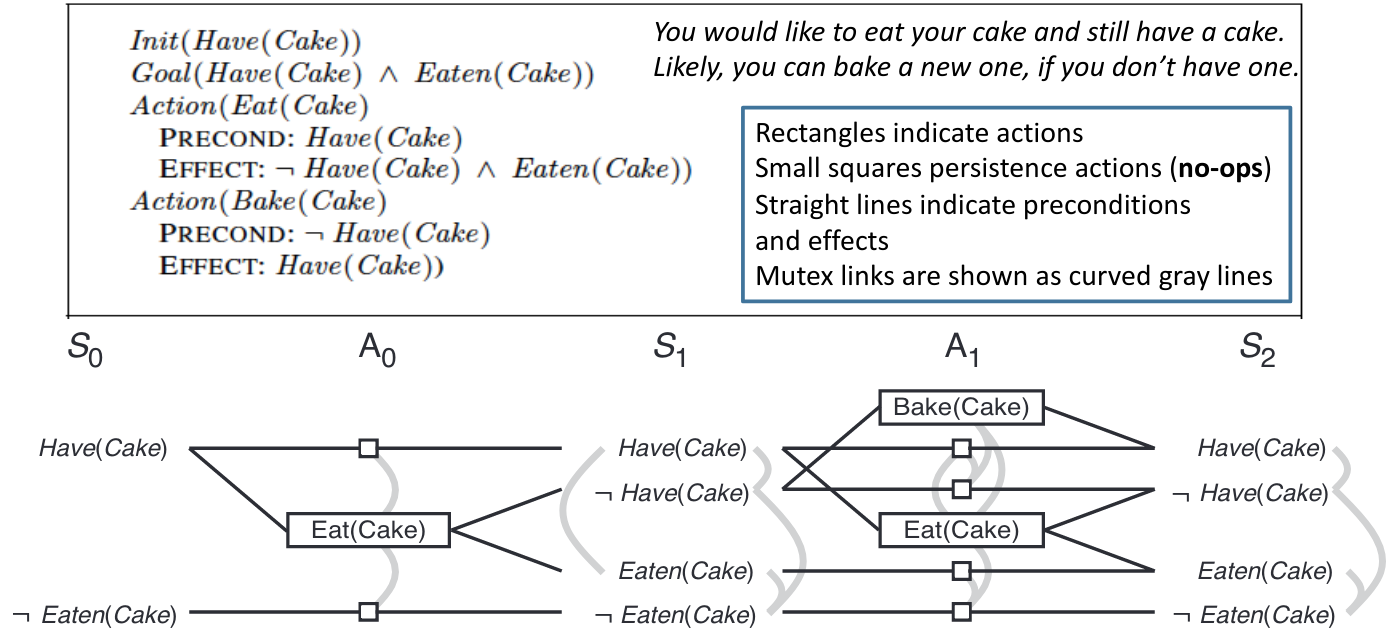
\includegraphics[width=\textwidth]{Images/examplePlanning}
	\caption{Example of Planning Graph}
	\label{img:examplePlanning}
\end{figure}
Each level $S_i$ represents a set of possible belief states and two literals connected by a mutex
belong to different belief states.\newline
The levels, alternating $S$'s an $A$'s, are computed until we reach a point where two consecutive
levels are identical.\newline
The level $j$ at which a literal first appears is never greater than the level at which it 
can be achieved and we call this the \emph{level cost} of a literal/goal.\newline
A planning graph is polynomial in the size of the planning problem: an entire graph with $n$ levels, $a$ actions, $l$ literals, has size $O(n (a + l)^2)$ also the time complexity is the same.

Planning graphs can provide useful informations, so we have that if any goal literal fails to 
appear in the final level of the graph, then the problem is unsolvable.\newline
We can estimate the cost of achieving a goal literal $g_i$ as by its level cost and a better
estimate can be obtained by serial planning graphs: by enforcing only one action at each level
(adding mutex).\newline 
Estimating the heuristic cost of a conjuction of goals can be done with $3$ heuristics:
\begin{description}
    \item [Max-level: ] the maximum level cost of any of the sub-goals and this is admissible.
    \item [Level Sum: ] the sum of the level costs of the goals and this can be inadmssible when
	                goals are not independent, but it may work well in practice.
    \item [Set Level: ] finds the level at which all the literals in the goal appear together in
	                the planning graph, without any mutex between pairs of them.\newline
			It is admissible, accurate but not perfect.
\end{description}
The planning graph can be seen as a relaxed problem with the following characteristics, so when
$g$ appears at level $S_i$ we can prove that if there exists a plan with $i$ action levels that
achieves $g$ then $g$ will appear at level $i$, and if $g$ does not appear there is no plan,
but not viceversa, so the fact that $g$ appears does not mean that there is a plan.

If $g$ does appear at level $i$, the plan possibly exists but to be sure we need to check the 
mutex relations, pairs of conflicting actions and pairs of conflicting literals.\newline
The \emph{GraphPlan} algorithm, with pseudocode in figure \ref{img:graphplan}, is a strategy
for extracting a plan from the planning graph, that can be computed incrementally 
by the function $\proc{Expand-Graph}$.\newline
Once a level is reached where all the literals in the goal show up as non-mutex, an attempt to
extract a plan is made with $\proc{Extract-Solution}$.\newline
If $\proc{Extract-Solution}$ fails, the failure is recorded as a no-good, another level is 
expanded and the process repeats until a termination condition is met.\newline
In figure \ref{img:exampleGraphPlan} is possible to see the graphplan on the spare-tire example.

\begin{figure}
	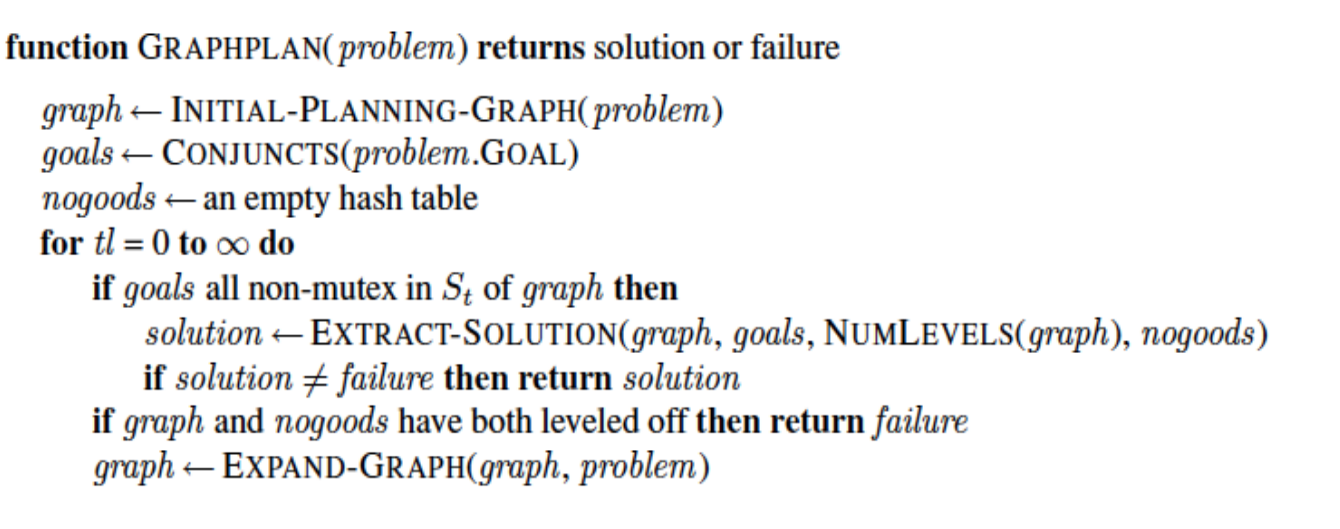
\includegraphics[width=\textwidth]{Images/graphplan}
	\caption{Pseudocode of $\proc{GraphPlan}$ algorithm}
	\label{img:graphplan}
\end{figure}

\begin{figure}
	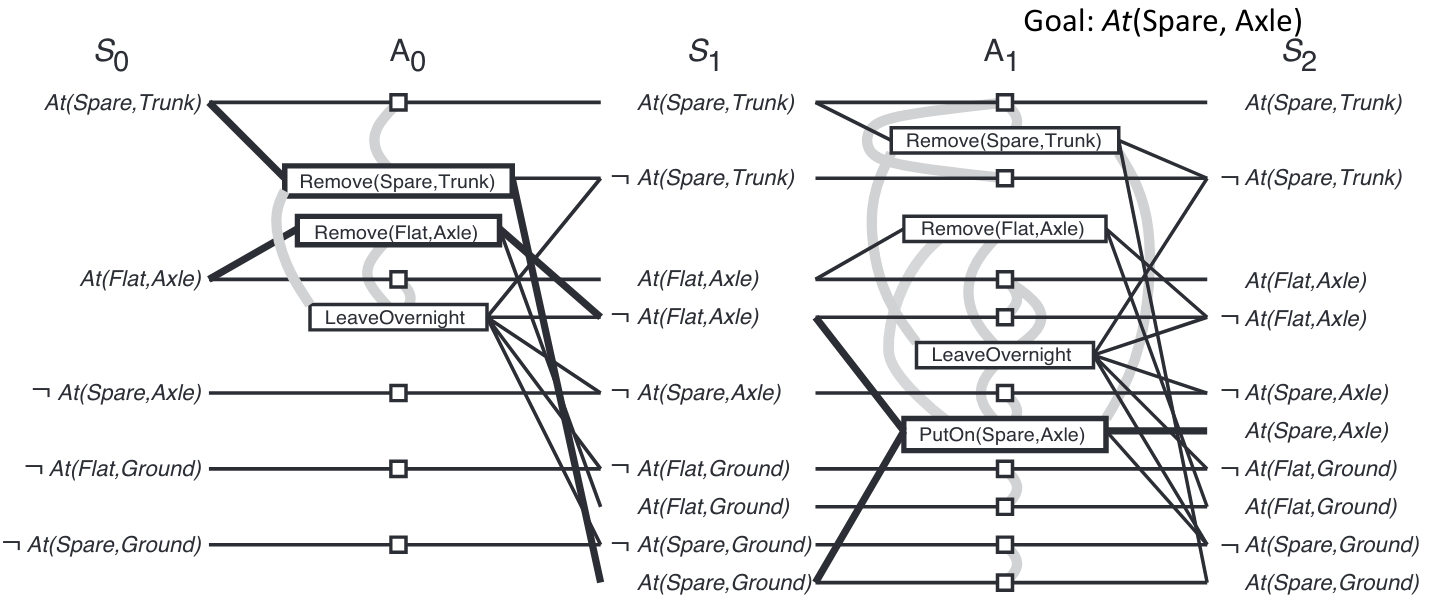
\includegraphics[width=\textwidth]{Images/exampleGraphPlan}
	\caption{Example of Graph Plan on the spare-tire problem}
	\label{img:exampleGraphPlan}
\end{figure}
To extract solution there are two approaches:
\begin{enumerate}
    \item Solve as a boolean CSP: the variables are the actions at each level, the values for 
	  each variable are in or out of the plan, and the constraints are the mutexes and the 
	  need to satisfy each goal and precondition.
    \item Solve as a backward search problem, we start with $S_n$ and the goal, and for each level
	  $S_i$ select a number of non-conflicting actions in $A_{i-1}$, whose effects cover the 
	  goals in $S_i$.\newline
	  The resulting state is $S_{i-1}$ with goals the preconditions of the selected actions
	  and the process is repeated until level $S_0$ hoping all the goals are satisfied.
\end{enumerate}
If $\proc{Extract-Solution}$ fails to find a solution for a set of goals at a given level, we 
record the $($level, goals$)$ pair as no-good, so that we can avoid to repeat the computation.

Constructing the planning graph takes polynomial time and solution extraction is intractable in
the worst case, but fortunately an heuristics exist.\newline
It is a greedy algorithm based on the level cost of the literals, which consist to pick first
the literal with the highest level cost and to achieve that literal, prefer actions with easier
preconditions, that is choose an action such that the sum (or maximum) of the level costs of 
its preconditions is smallest.

We can prove that $\proc{GraphPlan}$ will in fact terminate and return failure when there is no
solution, but we may need to expand the graph even after it levels off.\newline
\begin{thm}
    If the graph and the no-goods have both leveled off, and no solution is found we can 
    safely terminate with failure
\end{thm}
The sketch of the proof consist that literals and actions increase monotonically and are finite,
so we need to reach a level where they stabilize.\newline
Mutex and no-goods decrease monotonically and cannot become less that zero, so they too
must level off.\newline
When we reach this stable state if one of the goals is missing or is mutex with another goal
it will remain so we may as well stop computation.

We consider now other approaches for planning, starting from translating to a boolean SAT problem,
where we execute the following steps:
\begin{enumerate}
    \item Propositionalize the actions: create ground instances of the actions.
    \item Define the initial state $F^0$ for every fluent $F$ in the initial state, $\neg F^0$
	  for every fluent $F$ not in the initial state.
    \item Proposizionalize the goal, by instantiating variables to a disjunction of constants.
    \item Add successor-state axioms, so for each fluent we have 
	  \[ F^{t+1} \iff ActionCausesF^T \lor (F^t \land \neg ActionCausesNotF^t) \]
	  where $ActionCausesF^t$ is a disjunction of all the ground actions that have $F$ in 
	  their add list and $ActionCausesNotF^t$ is a disjunction of all the ground actions
	  that have $F$ in their delete list.
    \item Add precondition axioms, so for every ground action $A^t \Rightarrow PRE(A)^t$.
    \item Add action exlusion axioms, so every action is distinct from every other action.
\end{enumerate}
The resulting translation is in the form that can be given in input to SATPLAN to find a solution.

\emph{Partial Order Planning} is an interesting approach, very popular in the nineties, since 
it addresses the issue of independent subgoals can be performed in parallel.\newline
For some specific tasks, such as operations scheduling is the technology of choice and is 
interesting, because it represents a change of paradigm: planning as search in the state of
partial plans rather than in space of states and this refinement is also more explainable:
it makes easier for humans to understand what the planning algorithms are doing and 
verify that they are correct.\newline
The driving principle of POP is least commitment, and partially ordered plans do not order steps
in the plan unless necessary to do so, in a partial-order plan steps are partially ordered, and
also there is \emph{Plan linearization}, to impose a total order to a partially ordered plan.

Partially instantiated plans leave variables uninstantiated until is necessary to instantiate them
and a plan without variables is said to be totally instantiated.

Instead of searching in space of states as in the classical formulation, in POP we search in the
space of partial plans, so we start with an empty plan, at each step we use operators for plan 
construction and refinement (we can add actions, instantiate variables and add ordering constraints
between steps) and in the end we stop when we obtain a consistent and complete plan where 
all the preconditions of all the steps are satisfied and ordering constranits do not create cycles.

Partial plan are represented as a set of actions, among them Start and Finish, a set of open
preconditions and constraints among actions of two different types (Ordering relations $S_1 < S_2$
and causal links $S_1 \to _{cond} S_2$).\newline
In figure \ref{img:popActions} and \ref{img:emptyPop} is possible to note how actions are 
represented in POP approach and also how empty plan are represented.

\begin{figure}
	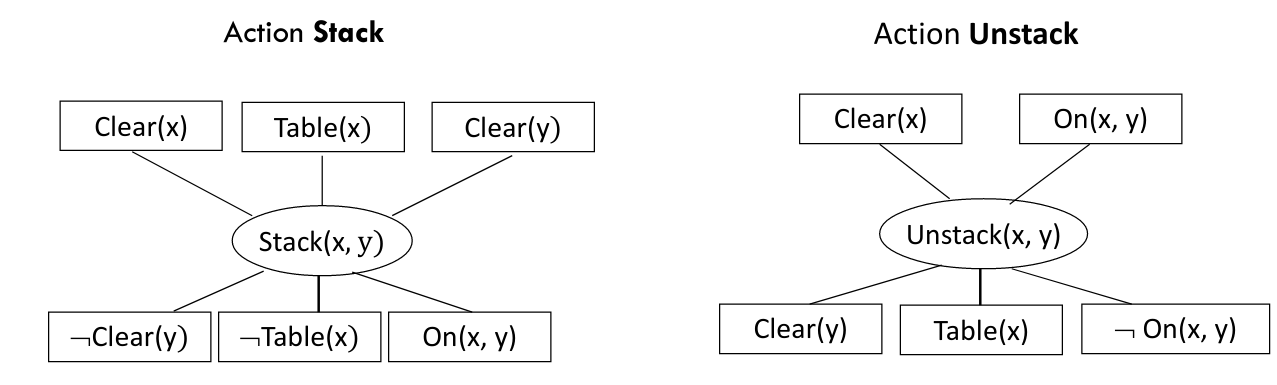
\includegraphics[width=\textwidth]{Images/popActions}
	\caption{Representation of POP actions}
	\label{img:popActions}
\end{figure}
\begin{figure}
	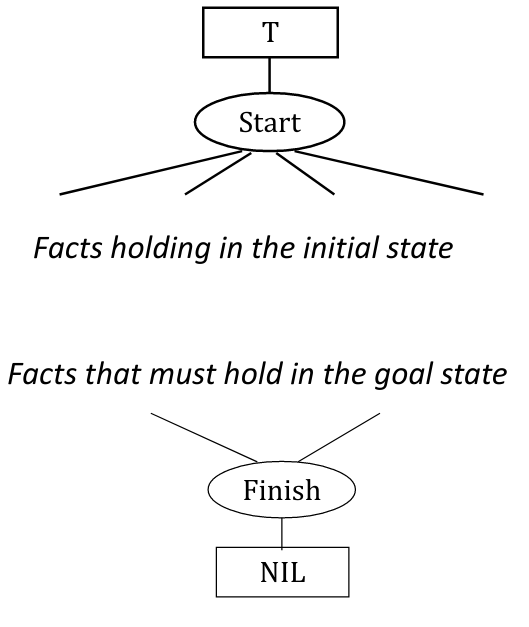
\includegraphics[width=\textwidth]{Images/emptyPop}
	\caption{Empty Plan on POP approach}
	\label{img:emptyPop}
\end{figure}
In POP algorithm we start with the empty plan, with Start and Finish, and at each step we 
choose a step $B$ and one of its open preconditions $p$ and we generate a successor plan for 
each action $A$ having $p$ among the effects.\newline
After choosing an action $A$ consistency is re-estabilished by add to the plan the constraints 
$A < B$ and $A \to_p B$, and possible actions $C$ having $\neg p$ as effect, are potential 
conflicts (or threats).\newline
They need to be anticipated or delayed by adding the constraints $C < A$ or $B < C$, and we 
stop when the set of open pre-conditions is empty.

In figure \ref{img:threats} is possible to see how we can remove threats and in figure 
\ref{img:POPExample} is possible to see POP in action.

\begin{figure}
	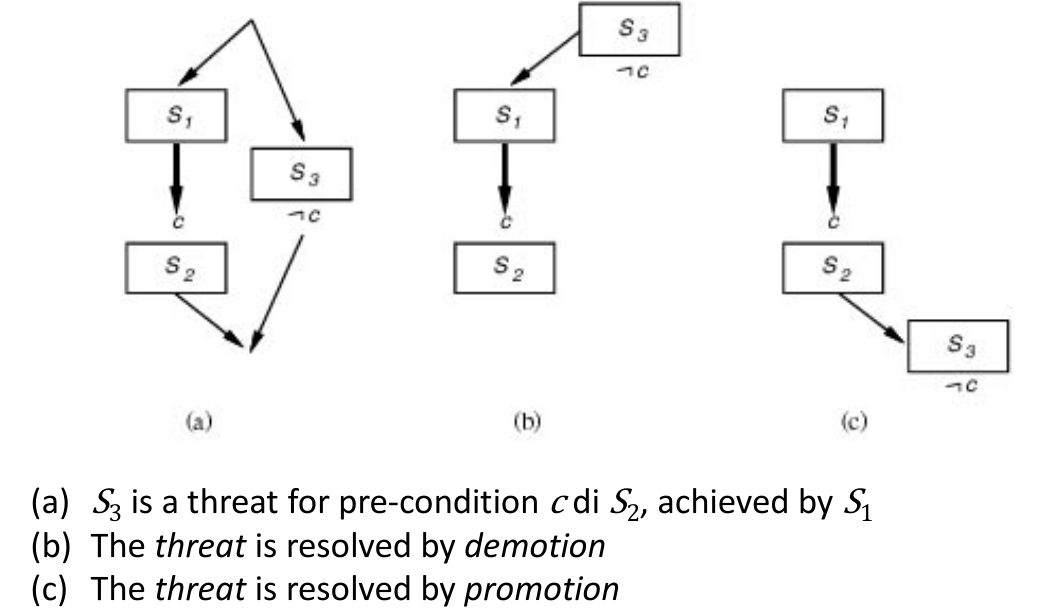
\includegraphics[width=\textwidth]{Images/threats}
	\caption{Example how to remove threats in POP}
	\label{img:threats}
\end{figure}
\begin{figure}
	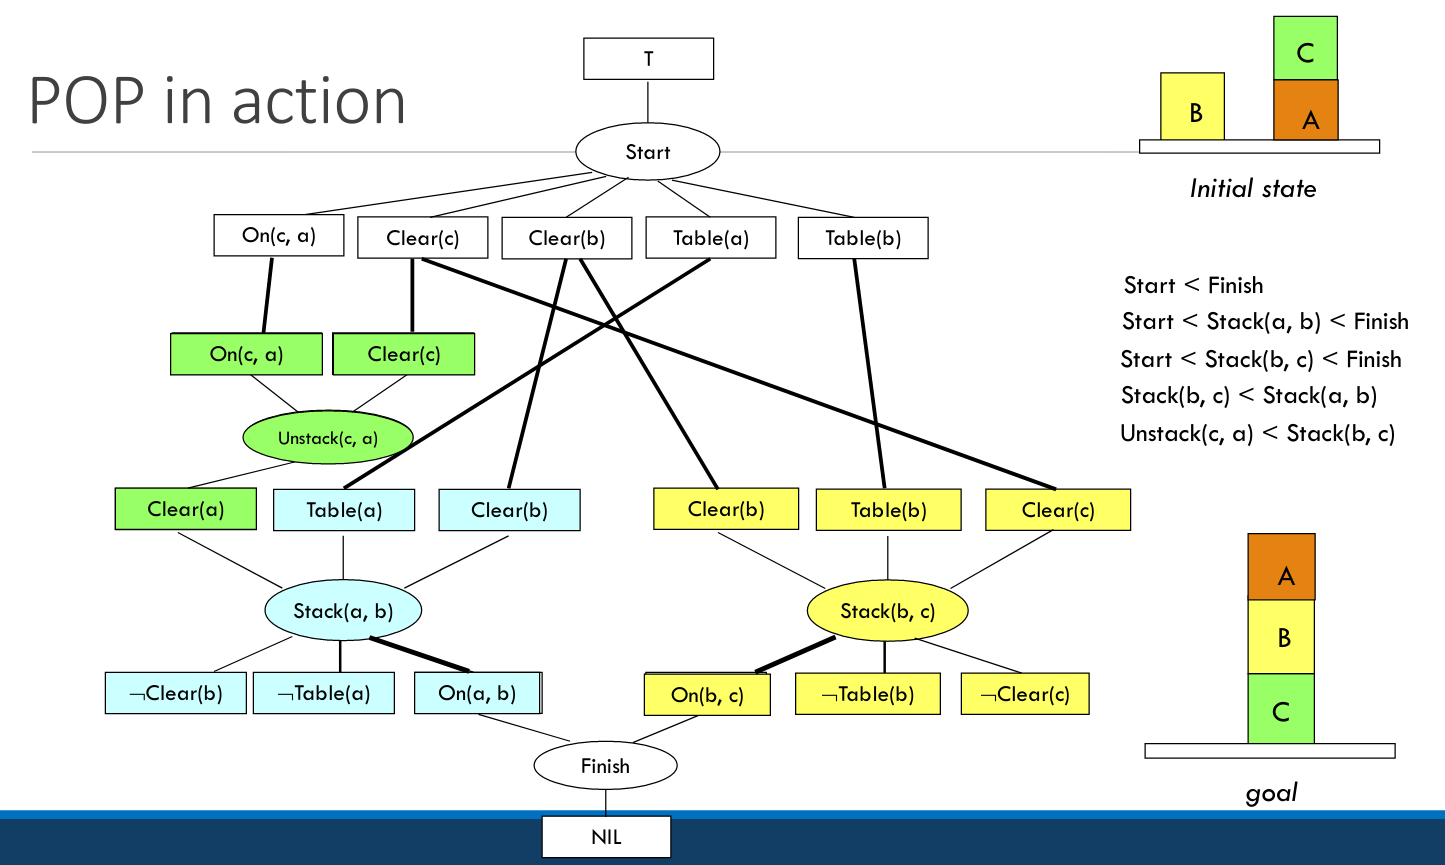
\includegraphics[width=\textwidth]{Images/POPExample}
	\caption{Example of POP in action}
	\label{img:POPExample}
\end{figure}
